\bookchapter{Kapitel 60: Entwicklungsumgebung einrichten – Xcode und das erste Projekt}

\chapterintro{Will der Handwerker gut arbeiten, muss sein Werkzeug scharf sein. In diesem Kapitel bauen wir die „Küche“ auf: Xcode installieren, den Simulator zum Laufen bringen, dein allererstes iOS-Projekt anlegen und die Projektstruktur auseinandernehmen, bis alles klar ist. Nach der Einrichtung wirst du zum ersten Mal sehen, wie dein eigener Code zu einem anklickbaren Button wird – diesen Moment behalten viele ein Leben lang.}

\booksection{Einen Mac besorgen}

Zuerst zur Hürde: iOS-Entwicklung läuft zwingend unter macOS. Ohne Mac hast du drei Optionen: einen kaufen (auch ein gebrauchter Mac mini oder ein MacBook Air genügt), kurzfristig einen Cloud-Mac mieten oder zuerst Teil 8 lesen, „Android-Entwicklung in der Praxis“ (das geht unter Windows).

\begin{center}
\begin{tabularx}{\linewidth}{|X|X|X|}
\hline
\textbf{Komponente} & \textbf{Minimum} & \textbf{Komfortzone (empfohlen)} \tabularnewline
\hline
Chip & Apple Silicon (ab M1) & M2 oder neuer \tabularnewline
Arbeitsspeicher & 8GB & 16GB \tabularnewline
Speicherplatz & 40 GB+ einplanen (Xcode selbst ist ein Brocken) & ab 256 GB \tabularnewline
System & das neueste macOS & automatische Updates aktiv lassen \tabularnewline
\hline
\end{tabularx}
\end{center}

\begin{center}\small\color{gray}Referenzkonfiguration für den Mac-Entwicklungsrechner (August 2026)\end{center}

\begin{tcbinfo}{Tipp: Auch ohne Mac kannst du schon die Sprache lernen}
Die kostenlose App Swift Playgrounds aufs iPad vermittelt die Swift-Grundlagen (kein Mac nötig); sie läuft sogar auf dem iPhone. Spiel die Sprachkenntnisse aus Kapitel 61 erst in Playgrounds ein – sobald der Mac da ist, geht es direkt durchstarten. „Ein scharfes Messer kostet Zeit, spart sie aber beim Hacken“ – genau das ist gemeint.

\end{tcbinfo}

\booksection{Xcode installieren}

Xcode ist Apples offizielle integrierte Entwicklungsumgebung – und kostenlos. In drei Schritten installiert:

\begin{enumerate}
  \item Auf dem Mac den App Store öffnen, nach „Xcode“ suchen und auf Installieren klicken – es sind etliche Gigabyte, such dir eine Zeit mit gutem Netz;
  \item Beim ersten Start die Vereinbarung akzeptieren und die Komponenten installieren (läuft automatisch);
  \item Im Menü Xcode Settings Locations prüfen, dass Command Line Tools ausgewählt ist – die Kommandozeilenwerkzeuge sind Voraussetzung für viele Skripte und Drittanbieter-Tools.
\end{enumerate}

\begin{tcbwarn}{Achtung: Version und System müssen zusammenpassen}
Ein neues Xcode verlangt oft das neueste macOS, alte Macs bleiben dann auf der alten Version hängen. Für die App-Store-Veröffentlichung verlangt Apple einen Build mit relativ aktuellem Xcode (meist mit einer Karenzzeit). Schiebe Systemupdates also nicht zu lange auf – iOS-Entwickler gehören zu den fleißigsten Verfolgern neuer Versionen.

\end{tcbwarn}

\booksection{Dein erstes Projekt anlegen}

Xcode öffnen Create New Project iOS wählen die App-Vorlage, dann ausfüllen:

\begin{center}
\begin{tabularx}{\linewidth}{|X|X|X|}
\hline
\textbf{Feld} & \textbf{Was eintragen} & \textbf{Erläuterung} \tabularnewline
\hline
Product Name & MyFirstApp & App-Name \tabularnewline
Team & Deine Apple ID (kostenlos) & Für die Signatur, ein persönliches Konto genügt \tabularnewline
Organization Identifier & com.example & Bildet mit dem Product Name die Paketkennung \tabularnewline
Interface & SwiftUI & Das Hauptframework dieses Buches \tabularnewline
Language & Swift & braucht keine Erklärung \tabularnewline
\hline
\end{tabularx}
\end{center}

\begin{center}\small\color{gray}Die fünf Einträge beim Anlegen eines Projekts\end{center}

Nach einem Klick auf Create erzeugt Xcode ein sofort lauffähiges Projekt. Wähle oben links einen Simulator (etwa iPhone 17) und drücke > – Sekunden später erscheint auf dem Simulatorbildschirm ein Fenster mit „Hello, world!“. Deine erste iOS-App ist geboren.

\booksection{Die Projektstruktur aufgeschlüsselt: was jede Datei macht}

Links ist der Projektnavigator; als Einsteiger brauchst du nur diese zu kennen:

\begin{center}
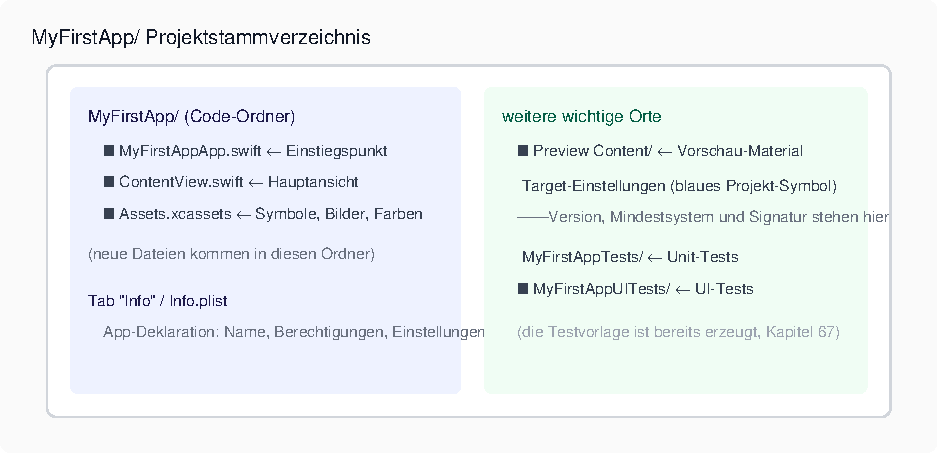
\includegraphics[width=0.92\linewidth]{figures/fig-di-liu-shi-zhang-1}
\\[2pt]\small Abbildung 2: Die Xcode-Projektstruktur, die Einsteiger kennen müssen
\end{center}

\begin{itemize}
  \item MyFirstAppApp.swift: der Programmeinstieg; in SwiftUI sind es nur ein paar Zeilen – „starten, dann die Hauptoberfläche zeigen“;
  \item ContentView.swift: die Hauptansicht; alles, was du gerade siehst, liegt hier;
  \item Assets.xcassets: das Ressourcenlager – Icons, Bilder und Farben liegen hier;
  \item Target-Einstellungen: über das blaue Projektsymbol links hinein; Versionsnummer, minimale iOS-Version und Signatur stehen dort. Auch Anzeigename und Icon der App konfigurierst du hier.
\end{itemize}

\booksection{Debugging auf dem echten Gerät: die App auf dein iPhone bringen}

\booksection{Xcode-Effizienztricks: die fünf „Tastenkürzel-Cheats“ für Einsteiger}

Wenn du diese beherrschst, wirkst du „sehr professionell“:

\begin{center}
\begin{tabularx}{\linewidth}{|X|X|X|}
\hline
\textbf{Aktion} & \textbf{Tastenkürzel} & \textbf{Wirkung} \tabularnewline
\hline
Ausführen & CmdR & Kompilieren und starten \tabularnewline
Canvas-Vorschau öffnen/umschalten & OptionCmd & Der Schalter für WYSIWYG \tabularnewline
Einrückung formatieren & CtrlI & Die Einrückung des ausgewählten Codes automatisch ordnen \tabularnewline
Datei schnell öffnen & CmdO & Dateinamen tippen, sofort offen (am häufigsten gebraucht!) \tabularnewline
Kommentieren/Kommentar aufheben & Cmd/ & Beim Debuggen Code nebenbei ein- und ausschalten \tabularnewline
\hline
\end{tabularx}
\end{center}

\begin{center}\small\color{gray}Die meistgenutzten Xcode-Tastenkürzel (das Einsteiger-Fünfer-Set)\end{center}

Zwei weitere versteckte Boni: mehrere Simulatoren gleichzeitig (iPhone und iPad nebeneinander laufen lassen, um Layouts zu vergleichen) und die Snippet-Bibliothek (häufige Codezeilen ins Snippets-Panel rechts ziehen, beim nächsten Mal per Knopfdruck einfügen) – nutz diese Effizienzwerkzeuge einfach, das Gefühl kommt von selbst.

\booksection{Debugging auf dem echten Gerät: die App auf dein iPhone bringen}

So gut der Simulator auch ist, das echte Gerät ist das Ziel. Auch mit einer kostenlosen Apple ID kannst du auf echten Geräten debuggen:

\begin{enumerate}
  \item iPhone per Datenkabel anschließen (oder kabellos im selben WLAN debuggen);
  \item In der Geräteliste oben in Xcode dein Handy wählen; beim ersten Mal wirst du zum Anmelden mit der Apple ID aufgefordert, die Signatur wird automatisch eingerichtet;
  \item Auf dem iPhone [Einstellungen] [Allgemein] [VPN \& Geräteverwaltung] deinem Entwicklerzertifikat vertrauen;
  \item > drücken, und die App landet auf dem echten Gerät.
\end{enumerate}

\begin{tcbwarn}{Achtung: die „Sieben-Tage-Grenze“ des kostenlosen Kontos}
Eine App mit Signatur einer kostenlosen Apple ID erlischt nach 7 Tagen (ein erneutes Ausführen verlängert die Gültigkeit). Das ist Apples Missbrauchsschutz und reicht für die Lernphase völlig; ein bezahltes Entwicklerkonto (99 US-Dollar pro Jahr) hat diese Grenze nicht, mehr dazu in Kapitel 67.

\end{tcbwarn}

\booksection{Erste Proben + Erste Hilfe bei häufigen Fehlern}

\booksection{Erste Proben + Erste Hilfe bei häufigen Fehlern}

Öffne ContentView.swift, ersetze den Text in Text(“Hello, world!”) durch deinen Namen und drücke CmdR – Sekunden später zeigt der Simulator deinen Namen. Glückwunsch: Du hast die erste vollständige Runde „Code ändern kompilieren installieren ausführen“ absolviert.

\begin{center}
\begin{tabularx}{\linewidth}{|X|X|X|}
\hline
\textbf{Fehlerbild} & \textbf{Häufige Ursache} & \textbf{Gegenmittel} \tabularnewline
\hline
Signing-Fehler & Kein Team gewählt, Zertifikat abgelaufen & In Target Signing dein Konto anhaken; beim kostenlosen Konto einmal neu ausführen \tabularnewline
Simulator bleibt schwarz/öffnet nicht & Beschädigtes Image & Menü Device Erase All Content; oder den Simulator löschen und neu anlegen \tabularnewline
Xcode lädt langsam/installiert nicht & Netzwerkschwankungen beim App Store & Andere Tageszeit wählen; oder das .xip-Offline-Paket von der Apple-Entwicklerseite laden \tabularnewline
\hline
\end{tabularx}
\end{center}

\begin{center}\small\color{gray}Erste-Hilfe-Tabelle für typische Einrichtungsfehler von Einsteigern\end{center}

\begin{tcbpractice}{Jetzt bist du dran: deine „Entwickler-Ritual“-Checkliste abschließen}
(1) Xcode installieren und den Simulator zum Laufen bringen; (2) die eigene App einmal auf dem echten Gerät starten und einen Screenshot als Erinnerung machen; (3) den Hello-Text durch deinen Namen ersetzen; (4) in den Target-Einstellungen den Anzeigenamen auf „Meine erste App“ ändern. Nach diesen vier Schritten bist du jemand mit einem eigenen Werk.

\end{tcbpractice}

\begin{tcbsummary}{Zusammenfassung des Kapitels}
\begin{itemize}
  \item Harte Hürden: Mac + Xcode; ohne Mac zuerst mit Swift Playgrounds auf dem iPad die Sprache lernen
  \item Xcode aus dem App Store installieren; neue Versionen verlangen neue Systeme, Updates nicht aufschieben
  \item Die fünf Elemente beim neuen Projekt: Name, Team, Organisationskennung, SwiftUI, Swift
  \item Projekt-Merksatz: Der Code liegt im Ordner MyFirstApp/; die Target-Einstellungen regeln Version und Signatur
  \item Beim Debuggen auf echten Geräten mit kostenloser Apple ID gilt die 7-Tage-Signaturgrenze; ein bezahltes Konto hat sie nicht
  \item Der Entwickleralltag = Code ändern CmdR Ergebnis ansehen, im ewigen Kreislauf
\end{itemize}

\end{tcbsummary}
